\documentclass[12pt,fleqn]{article}

\title{Graphing better Impulse Response Functions for discrete-time
  linear models}

\author{Gray Calhoun\thanks{Economics Department; Iowa State
    University; Ames, IA 50011. Telephone: (515) 294-6271.  Email:
    \guillemotleft gcalhoun@iastate.edu\guillemotright, web:
    \guillemotleft http://www.econ.iastate.edu/\textasciitilde
    gcalhoun\guillemotright.} \\
  Iowa State University}

% The LaTeX macros in this file are available through the CC0 license
% (creative commons public domain.  See
% <http://creativecommons.org/publicdomain/zero/1.0> for more
% details.)  To the extent possible under law, the copyright holders
% have waived all copyright and related or neighboring rights to the
% contents of this file.

\usepackage[letterspace=35]{microtype}
\newcommand{\allcaps}[1]{\textls{\MakeUppercase{#1}}}

\newcommand{\AIC}{\allcaps{AIC}}
\newcommand{\BIC}{\allcaps{BIC}}
\newcommand{\BRC}{\allcaps{BRC}}
\newcommand{\CDF}{\allcaps{CDF}}
\newcommand{\CLT}{\allcaps{CLT}}
\newcommand{\DGP}{\allcaps{DGP}}
\newcommand{\FCLT}{\allcaps{FCLT}}
\newcommand{\FWE}{\allcaps{FWE}}
\newcommand{\GDP}{\allcaps{GDP}}
\newcommand{\HAC}{\allcaps{HAC}}
\newcommand{\IRF}{\allcaps{IRF}}
\newcommand{\IRFs}{\allcaps{IRF}s}
\newcommand{\LLN}{\allcaps{LLN}}
\newcommand{\LM}{\allcaps{LM}}
\newcommand{\MA}{\allcaps{MA}}
\newcommand{\MDS}{\allcaps{MDS}}
\newcommand{\MSE}{\allcaps{MSE}}
\newcommand{\NBER}{\allcaps{NBER}}
\newcommand{\NSF}{\allcaps{NSF}}
\newcommand{\NED}{\allcaps{NED}}
\newcommand{\OLS}{\allcaps{OLS}}
\newcommand{\OOS}{\allcaps{OOS}}
\newcommand{\SFWE}{\allcaps{SFWE}}
\newcommand{\SPA}{\allcaps{SPA}}
\newcommand{\VAR}{\allcaps{VAR}}
\newcommand{\WFWE}{\allcaps{WFWE}}

% Check if shell commands can be executed
\ifnum\pdfshellescape=1
% Yes, enabled
\newcommand{\VERSION}{\splice{echo `git log -1 --date=short --format=\%cd`, `git describe --dirty`}}
\else
% No, disabled
\providecommand\VERSION{\today}
\fi
\date{\VERSION}
\usepackage{amsmath}
\usepackage{lucidabr}
\usepackage[margin=1in]{geometry}
\usepackage{
    amsfonts,
    amssymb,
    amsthm,
    bashful,
    bm,
    booktabs,
    enumitem,
    fancyhdr,
    flexisym,
    graphicx,
    mathtools,
    ragged2e,
    sectsty,
    setspace,
    slantsc,
    tabularx,
    tocstyle,
    url,
}
\allsectionsfont{\normalsize\RaggedRight}

\urlstyle{same}
\newcolumntype{C}{>{\centering\arraybackslash}X}

\pagestyle{fancy}
\renewcommand{\sectionmark}[1]{\markboth{}{\footnotesize{\thesection. #1}}}
\renewcommand{\subsectionmark}[1]{\markboth{}{\footnotesize{\thesubsection. #1}}}
\renewcommand{\headrulewidth}{0pt}
\renewcommand{\footrulewidth}{0pt}
\fancyhead[LE,LO]{\textit{\footnotesize{\nouppercase{\rightmark}}}}
\rhead{\footnotesize{\textit{\VERSION}}}

\onehalfspacing

\usepackage[small]{caption}
\usepackage[T1]{fontenc}
\usepackage[letterspace=35]{microtype}
\usepackage[sort,round,comma]{natbib}
\bibliographystyle{abbrvnat}
\newcommand\citepos[2][]{\citeauthor{#2}'s \citeyearpar[#1]{#2}}
\newcommand\poscw{\citeauthor{ClW:06}'s \citeyearpar{ClW:06,ClW:07}}
\newcommand\citen[1]{\citeauthor{#1}, \citeyear{#1}}

\newtheorem{proposition}{Proposition}

\renewcommand{\Re}{\operatorname{Re}}
\renewcommand{\Im}{\operatorname{Im}}

\DeclareMathOperator{\whitenoise}{\mathit{white\ noise}}
\DeclareMathOperator{\E}{E}
\DeclareMathOperator{\floor}{floor}
\DeclareMathOperator{\ceil}{ceil}

\newcommand{\vep}{\varepsilon}
\newcommand{\AR}{\allcaps{AR}}
\newcommand{\RR}{\mathbb{R}}
\newcommand{\VECM}{\allcaps{VECM}}

\newcommand{\Fs}{\mathcal{F}}

%%% Local Variables:
%%% mode: latex
%%% TeX-master: "../smoothirf.tex"
%%% TeX-command-extra-options: "-shell-escape"
%%% End:


\begin{document}
\maketitle
\begin{abstract}\noindent%
  We show how to construct continuous and differentiable
  Impulse Response Functions and for discrete-time Vector Autoregressions
  and Vector Error-Correction Models. Current methods produce piecewise linear
  functions that introduce visual distortions, especially when many
  response functions are plotted in the same graph to represent
  uncertainty or partial identification. We also show how to plot the
  cumulative response to a shock. In addition to being more accurate
  than current methods, our proposed approach is also much more attractive.
\end{abstract}

\tableofcontents
\newpage

\section{Introduction}
\label{S1}

Impulse Response Functions (\IRF s) are widely used in macroeconomics
to represent the dynamic effect over time of an unanticipated shock to
an economic system. If $y_t$ is a stationary sequence of random
vectors, an \IRF\ is a graph of the change in the conditional
expectation of $y_{t+s}$ in response to an unanticipated shock to
$y_t$, plotted as a function of $s$. The conditional expectation may
be implied by a theoretical model or a statistical model, such as a
\VAR, in which case additional assumptions may be necessary to
identify the shocks of interest. In either of these cases, \IRF s
provide a parsimonious and interpretable summary of the key features
of the model.

Producing an \IRF\ requires calculating the conditional expectation
$\E_t y_{t+s}$ under different counterfactual scenarios; with and
without the shock of interest. Since most macroeconomic models are
defined and estimated in discrete time (both $t$ and $s$ are
integers) the conditional expectations used to produce \IRF s are
calculated in discrete time as well. (See Chapter 1 of
\citealp{Ham:94}, for example.) But in most applications, it is
desireable to graph the \IRF s as curves and connect the points; this
is especially important when more than one \IRF\ is plotted on the
same graph --- whether to represent dynamics under different
assumptions (see \citealp{BeM:98}, and \citealp{StW:01}, for
representative examples), to represent statistical uncertainty
(\citealp{Kil:98}, and \citealp{SiZ:99}) or to represent regions that
are partially identified (\citealp{Uhl:05}, and
\citealp{InK:13}). Currently, this is done by linear interpolation
between the integer values of $\E_t y_{t+s}$. Unfortunately, this
practice has some drawbacks: linear interpolation introduces
misleading visual distortions and can remove potentially interesting
dynamics from the model.

In this paper, we show how \IRF s can be meaningfully defined for
vector ARMA and other linear time series models for all values of $t$
and $s$, even noninteger values. This allows researchers to use the
model itself to interpolate between the integers and ensures that the
interpolation obeys the same dynamics as the rest of the model. The
resulting graph removes the distortions introduced by current methods.
Section~\ref{S2} presents these results, Section~\ref{S3} provides
some numeric and empirical examples, and Section~\ref{S4} concludes.

\section{Finite-order linear models}
\label{S2}

This section presents the main results of the paper: smooth \IRF s for
finite-order linear models. Section~\ref{S2.1} presents results for
the AR(1) to motivate our approach. Section~\ref{S2.2} extends this
result to finite-order \VAR s and Section~\ref{S2.3} extends the
result further to VARMA and VECM models and to cumulative responses.
The rest of this subsection introduces some notation and defines the
\IRF s.

Let $\{y_t\}$ be a stationary sequence of random vectors in $\RR^k$,
let $\Fs_t$ represent the information set available in period $t$,
\begin{equation*}
  \Fs_t = \sigma(y_t, y_{t-1}, y_{t-2},\dots),
\end{equation*}
and let $\E_t$ denote the conditional expectation
$\E(\cdot \mid \Fs_t)$. Assume for now that $\E_t y_{t+s}$ for
nonnegative $s$ only depends on $y_t,\dots,y_{t-p}$ for a finite value
of $p$ and let the function $m_s$ represent this conditional
expectation of $y_{t+s}$, so
\begin{equation*}
  m_s(x_0,\dots,x_p)
  = \E(y_{t+s} \mid y_t = x_0,\dots, y_{t-p} = x_p)
\end{equation*}
for each $s \geq 0$. For later convenience, define $m_s = 0$ for
$s < 0$ and let $\E y_t = \mu$. For a shock of theoretical interest
$u$, with $u \in \RR^k$, the \IRF\ corresponding to $u$ is the
difference
\[
  \Psi_u(s) =
  m_s(\mu + u, \mu, \dots, \mu) - m_s(\mu, \mu, \dots,\mu).
\]
Often theoretical shocks are normalized so that $\lvert u \rvert = 1$
but that is not necessary.

If $y_t$ is nonstationary $\E_t$ may depend on the value of $t$. In that
case, define
\begin{equation*}
  m_{ts}(x_0,\dots,x_p)
  = \E(y_{t+s} \mid y_t = x_0,\dots, y_{t-p} = x_p)
\end{equation*}
and let
\begin{equation*}
  \Psi_{tu}(s) =
  m_{ts}(\E y_t + u, \E y_{t-1}, \dots, \E y_{t-p}) - m_{ts}(\E y_t, \E y_{t-1}, \dots,\E y_{t-p}).
\end{equation*}
Note that $\Psi_{tu}$ can be independent of $t$ even if $m_{ts}$ is
not.

\subsection{Motivation with an AR(1)}
\label{S2.1}

\begin{figure}[t]
  \centering
  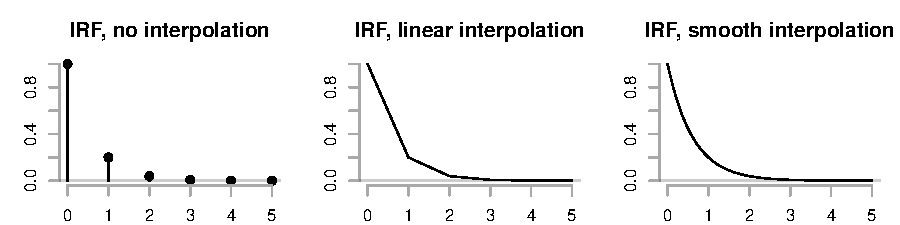
\includegraphics{graphs/motivation.pdf}
  \caption{\IRF\ for simple AR(1) example. Here $y_t = 0.2 y_{t-1} +
    \vep_t$ --- the vertical axis shows $\Psi_1(x)$. The left panel
    plots only integer values of $x$, the middle panel uses linear
    interpolation between the integers, and the right panel plots the
    function $0.2^x$ directly.}
  \label{fig:1}
\end{figure}

For motivation, start with the simplest univariate case and assume
that $y_t$ is the \AR(1)
\begin{equation}
  \label{eq:1}
  y_t = a y_{t-1} + \vep_t
\end{equation}
where $\vep_t$ is a martingale difference sequence and
$\lvert a \rvert < 1$.  For discrete-time models, it is easy to define
the \IRF\ recursively and $\Psi_h(s) = a^s u$. When $a > 0$, this
function is well-defined for all positive real $s$, and can be used
directly to interpolate between the integer points. But typically
representing these dynamics has been achieved by linear interpolation,
so
\begin{align}
  \label{eq:2}
  \Psi_u(s)
  &= (s - \lfloor s\rfloor) \Psi_u(\lfloor s\rfloor+1)
    + (1 - s + \lfloor s\rfloor) \Psi_u(\lfloor s\rfloor) \\
  \label{eq:3}
  &= (s - \lfloor s\rfloor) a^{\lfloor s \rfloor + 1} u
    + (1 - s + \lfloor s\rfloor) a^{\lfloor s \rfloor} u
\end{align}
for noninteger $s$, where $\lfloor s\rfloor$ is the largest integer
less than or equal to $s$.

Figure~\ref{fig:1} plots $\Psi_u(s)$ for $u = 1$ and $a = 0.2$ using
three approaches: first only for the integer values of $s$, second
using linear interpolation between the integer values defined
by~\eqref{eq:3}, and finally using $a^s u$ directly for all
$s \geq 0$.\footnote{%
  All of the graphs in this paper were produced using R. \citep{R}} %
While one could debate which of the functions represents the `true'
impact of a shock at a fractional point in time and whether the
interpolated points should be interpreted, the dynamics and rate of
decay of the AR model are much more clearly represented by the right
panel that graphs $0.2^s$ directly.

This should not be surprising. We can see that $\Psi_u(s) = a^s u$
satisfies the recurrence relation implied by the lag structure of the
original \AR\ process for any positive real value of $s$:
\begin{equation}
  \label{eq:4}
  \Psi_u(s) = a^s u = a \times a^{s-1} u = a \, \Psi_u(s-1).
\end{equation}
Letting $\Phi(L)$ define the lag polynomial of the \AR(1) defined by
Equation~\eqref{eq:1}, (so the autoregressive model is defined as
$\Phi(L)y_t = \vep_t$ for all $t$) we can express~\eqref{eq:4} in a
form that will be easier to extend to more complicated \DGP s,
\begin{equation}
  \label{eq:5}
  \Phi(L) \Psi_u(s) = 0
\end{equation}
for all $s \in \RR^+$ with the implicit definition
$L \Psi_u(s) = \Psi_u(s-1)$. When $\Psi_u(s)$ is constructed by linear
interpolation, i.e.~\eqref{eq:3}, the recursive
relationships~\eqref{eq:4} and~\eqref{eq:5} only hold for integer
values of $s$.

\begin{figure}[t]
  \centering
  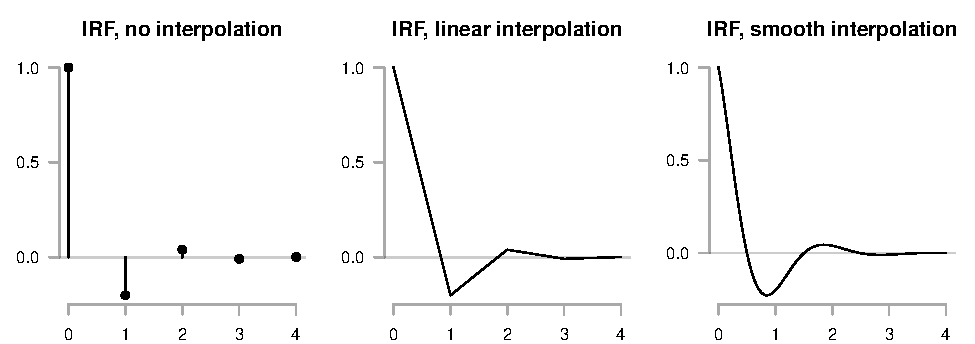
\includegraphics{graphs/motivation2.pdf}
  \caption{\IRF\ for simple AR(1) example. Here $y_t = -0.2 y_{t-1} +
    \vep_t$ --- the vertical axis shows $\Psi_x(1)$. The left panel
    plots only integer values of $x$, the middle panel uses linear
    interpolation between the integers, and the right panel plots the
    function $|a|^x \cos(\pi x)$ directly.}
  \label{fig:2}
\end{figure}

The case $a \in (-1, 0)$ is slightly more complicated.  The previous
solution, $a^s u$, is well-defined and real-valued only for integer
values of $s$, so it can no longer be used directly for interpolation
between the noninteger points. Instead, we consider the definition
\begin{equation}
  \Psi_u(s) = |a|^s \cos(\pi s) \cdot u.
\end{equation}
This function is exactly equal to $a^s u$ for nonnegative integer
values of $s$ and is well-defined and real valued for noninteger $s$.
Moreover, this $\Psi_u(s)$ satisfies the recurrence relation for the
\AR(1) model for all values of $a \in (-1,1)$
\begin{equation*}
  \Psi_u(s) = |a|^s \cos(\pi s) \cdot u = - |a| \times |a|^{s-1} \cos(\pi (s-1)) \cdot u = a \, \Psi_u(s-1)
\end{equation*}
implying that
\begin{equation*}
  (1 - a L) \, \Psi_u(s) = 0
\end{equation*}
as before. Figure~\ref{fig:2} plots the \IRF s for $a = -0.2$ and
$u = 1$ with no interpolation, linear interpolation, and the
definition of $\Psi_u(s)$. Just as before, the smooth version more
accurately reflects the system's dynamics after a shock.

This choice of $\Psi_u(s)$ was not made at random. Any complex
number $a + bi$ can be written in polar form,
\[
a + bi = R [\cos(\theta) - i \sin(\theta)]
\]
where $R = |a^2 + b^2|^{1/2}$ and $\theta$ satisfies
$\cos(\theta) = a/R$ and $\sin(\theta) = b/R$. Real powers of $a + bi$
can be expressed as\footnote{%
  See \citet{Ham:94} for background on complex numbers.} %
\[
(a + bi)^s = R^s [\cos(\theta s) - i \sin(\theta s)].
\]
For the \AR\ example above, $a < 0$ and $b = 0$ so $\theta = \pi$.
Then $a^s = |a|^s \cos(\pi s)$ as we originally claimed. This example
also suggests a more general method for interpolating between integer
values of $s$ for any \VAR; solve recurrence relation using standard
tools (as described in \citealp{Ham:94}, for example) and use the
solution as the \IRF\ for real-valued $s$. We pursue that approach in
the next section.

\subsection{General Approach for VAR(\textit{p})}
\label{S2.2}

The \AR(1) model in the previous section can be extended to general
\VAR s using the ``canonical'' representation.\footnote{%
  See Chapter 1 of \citet{Ham:94} for a textbook treatment of much of
  this material.} %
Define $y_t$ to be the \VAR($p$),
\[
y_t = \sum_{j=1}^p A_j y_{t-j} + \vep_t.
\]
(We assume that $y_t$ has mean zero to simplify notation without loss
of generality.) To represent this relationship as a \VAR(1), form the
vector $(y_t',\dots,y_{t-p+1}')'$ and observe that
\begin{equation}
\label{eq:6}
\underbrace{\begin{pmatrix*}[l]
  y_t \\ y_{t-1} \\ y_{t-2} \\ \vdots \\ y_{t-p+1}
\end{pmatrix*}}_{Z_t}
=
\underbrace{\begin{pmatrix*}[l]
  A_1 & A_2 & \cdots & A_{p-1} & A_p \\
  I_k & 0   & \cdots & 0 & 0 \\
  0  & I_k  & \cdots & 0 & 0 \\
  \vdots & \vdots & \ddots & \vdots & \vdots \\
  0 & 0 & \cdots & I_k & 0
\end{pmatrix*}}_{F}
\underbrace{\begin{pmatrix*}[l]
  y_{t-1} \\ y_{t-2} \\ y_{t-3} \\ \vdots \\ y_{t-p}
\end{pmatrix*}}_{Z_{t-1}}
+
\underbrace{\begin{pmatrix*}[l]
  \vep_{t} \\ 0 \\ 0 \\ \vdots \\ 0
\end{pmatrix*}}_{U_t}.
\end{equation}
So this relationship is equivalent to $Z_t = F Z_{t-1} + U_t$. The
conditional expectation has a convenient form that is trivial to
calculate for integer values of $s$,
\begin{equation*}
  m_s(x) = e_1 F^s x
\end{equation*}
where $e_1$ is the selection matrix
\begin{equation*}
  e_1 = \begin{pmatrix*}[l]
    I_k & 0 & \cdots & 0
  \end{pmatrix*}.
\end{equation*}
Consequently, the \IRF\ has the form
\begin{equation*}
  \Psi_u(s) = e_1 F^s u_0
\end{equation*}
for integer values of $s$, where we define $u_0$ to be the vector
$(u', 0)'$. This section will show that a variation of this definition
remains meaningful for noninteger values of $s$.

Suppose that $F$ has $q$ distinct eigenvalues. Then $F$ can be
decomposed as
\[
F = M J M^{-1}
\]
where $J$ is block diagonal of the form
\[
J = \begin{pmatrix*}[l]
  J_1 & \cdots & 0 \\
  \vdots & \ddots & \vdots \\
  0 & \cdots & J_q
\end{pmatrix*}.
\]
Each $J_\ell$ is an $n_\ell \times n_\ell$ of the form
\[
J_\ell =
\begin{pmatrix*}[l]
  \lambda_\ell & 1 & 0 & \cdots & 0 & 0 \\
  0 & \lambda_\ell & 1 & \cdots & 0 & 0 \\
  0 & 0 & \lambda_\ell & \cdots & 0 & 0 \\
  \vdots & \vdots & \vdots & \ddots & \vdots & \vdots \\
  0 & 0 & 0 & \cdots & \lambda_\ell & 1 \\
  0 & 0 & 0 & \cdots & 0 & \lambda_\ell
\end{pmatrix*}
\]
where $\lambda_1,\dots,\lambda_q$ are the distinct eigenvalues of $F$
and $n_\ell$ is the number of times the $\ell$th eigenvalue is
repeated.  If all of the eigenvalues of $F$ are distinct, this is just
the eigenvalue decomposition of $F$.

This representation is convenient because, for positive integer values
of $s$, we have
\[
F^s = M J^s M^{-1}
\]
and
\begin{align*}
J^s =
\begin{pmatrix*}[l]
  J_1^s  & \cdots & 0      \\
  \vdots & \ddots & \vdots \\
  0      & \cdots & J_q^s
\end{pmatrix*}, &&
J_\ell^s &=
\begin{pmatrix*}[l]
  h_\ell(s,0) & h_\ell(s,1) & h_\ell(s,2) & \cdots & h_\ell(s,n_\ell)   \\
  0           & h_\ell(s,0) & h_\ell(s,1) & \cdots & h_\ell(s,n_\ell-1) \\
  0           & 0           & h_\ell(s,0) & \cdots & h_\ell(s,n_\ell-2) \\
  \vdots      & \vdots      & \vdots      & \ddots & \vdots             \\
  0           & 0           & 0           & \cdots & h_\ell(s,0)        \\
\end{pmatrix*},
\end{align*}
  where $h_\ell(s,j)$ is defined as
\begin{equation*}
h_\ell(s,j) =
\begin{cases}
  |\lambda_\ell|^s \big[\cos(\theta_\ell s) + i \sin(\theta_\ell s)\big] & j = 0 \\
  \frac{s!}{j!(s-j)!} |\lambda_\ell|^s \big[\cos(\theta_\ell s) + i \sin(\theta_\ell s)\big] & \text{if } s \geq j > 0 \\
  0 & \text{otherwise.}
\end{cases}
\end{equation*}
and $\theta_\ell$ satisfies
$\cos(\theta_\ell) = \Re(\lambda_\ell)/|\lambda_\ell|$ and
$\sin(\theta_\ell) = \Im(\lambda_\ell)/|\lambda_\ell|$ as before.

This representation allows us to write
\begin{multline}
  \label{eq:7}
  F^s =
  \sum_{j = 1}^q \sum_{l=0}^{\min(n_\ell, \lfloor s\rfloor)} \tfrac{s(s-1)\cdots(s-l+1)}{l (l - 1) \cdots 1} |\lambda_j|^{s-l} \\
  \times\Big\{\big[B_{jl} \cos(\theta_j s) + C_{jl} \sin(\theta_j s)\big] + i\big[D_{jl} \cos(\theta_j s) + E_{jl} \sin(\theta_j s)\big]\Big\}
\end{multline}
where the coefficient matrices $B_{jl}$, $C_{jl}$, $D_{jl}$, and
$E_{jl}$ are chosen to match $F^0, F^1, F^2,\dots$. For integer
values of $s$, the imaginary components of $M J^s M^{-1}$ exactly
cancel, so we can use the real part of~\eqref{eq:7} alone, giving
\begin{equation}
  \label{eq:8}
  F^s =
  \sum_{j = 1}^q \sum_{l=0}^{\min(n_\ell, \lfloor s \rfloor)} \tfrac{s(s-1)\cdots(s-l+1)}{l (l - 1) \cdots 1} |\lambda_j|^{s-l} \big[B_{jl} \cos(\theta_j s) + C_{jl} \sin(\theta_j s)\big]
\end{equation}
to produce $F^1, F^2, F^3,\dots$. Our proposal, in a nutshell, is to
use the definition given by~\eqref{eq:8} for all of the reals rather
than just the integers, exactly as we did in the motivating \AR(1)
examples.

Equation~\eqref{eq:7} has another practical implication. Although
$F^s$ has real and imaginary components for real $s$, we are only
interested in its real component, which generates the \IRF s for
integer values of $s$. Rather than calculating the matrices $B_{jl}$
and $C_{jl}$ to use~\eqref{eq:8}, we can calculate the complex valued
$F^s$ and simply drop its imaginary component. This calculation is
directly available in many programming languages and can be
implemented as $M J^s M^{-1}$ using the Jordan decomposition if it is
not.

We conclude this section with a formal statement of the result.

\begin{proposition}[Impulse Response Functions for \VAR s]
  \label{P1}
  Let $F$ be the coefficient matrix of the canonical \VAR(1)
  representation of an arbitrary real-valued \VAR($p$). Define
  $\Psi_u(s) = e_1 \Re(F^s) u_0$ for all $s \in [0,+\infty)$, where
  $u_0 = (u', 0')'$ for some shock $u$ of theoretical interest. Then
  $\Psi_u(s) = m_s(\mu + u, \dots, \mu) - m_s(\mu,\dots,\mu)$ for all
  integer values of $s$ and $\Psi_u(s)$ satisfies the recurrence
  relation implied by the original \VAR,
  \begin{equation}
    \label{eq:9}
    \Psi_u(s) = \sum_{j=1}^q A_j \Psi_u(s-j)
  \end{equation}
  for all $s > 0$.
\end{proposition}
\begin{proof}
  The fact that $\Psi_u(s)$ meets the definition of the \IRF\ on
  integers is discussed in the text and follows from well-known
  algebra. Observe that the series $a_s = \Re(F^s) u_0$ satisfies
  $a_s = F a_{s-1}$ since $F$ is real and
  \[
    F a_{s-1} = F \Re(F^{s-1}) u_0
    = \Re(F^s) u_0
    = a_s.
  \]
  The conclusion of this proposition is a direct consequence.
\end{proof}

\subsection[Finite-order linear models]{Extensions to other finite-order linear models}
\label{S2.3}

This section considers three extensions to the previous section.
First, we show how to calculate cumulative response functions for
\VAR($p$)s. Second, we show how to calculate \IRF s for Vector Error
Correction Models (\VECM). Third, we show how to calculate \IRF s for
VARMA($p$, $q$) models. These results all rely on augmenting the
series to create a new canonical \VAR(1) and can easily be combined
and extended further.

First, suppose that $y_t$ has a \VAR($p$) representation as before.
but we want to derive the effect of the shock $u$ on $S_t$, the
cumulative sum of the $y_t$'s,
\[
  S_t = \sum_{s=0}^t y_s.
\]
Since $S_t - y_t = S_{t-1}$, we can extend the canonical
representation for $y_t$ by embedding this relationship as the first
element of the vector $Z_t$ in~\eqref{eq:6}. Equation~\eqref{eq:6}
becomes
\begin{equation*}
  \begin{pmatrix*}[l]
    S_t - y_t \\ y_t \\ y_{t-1} \\ \vdots \\ y_{t-p+1}
  \end{pmatrix*}
  =
  \begin{pmatrix*}[l]
    I      & 0      & \cdots & 0       & 0      \\
    0      & A_1    & \cdots & A_{p-1} & A_p    \\
    0      & I      & \cdots & 0       & 0      \\
    \vdots & \vdots & \ddots & \vdots  & \vdots \\
    0      & 0      & \cdots & I       & 0
  \end{pmatrix*}
  \begin{pmatrix*}[l]
    S_{t-1}  \\ y_{t-1} \\ \vdots \\ y_{t-p+1} \\ y_{t-p}
  \end{pmatrix*}
  +
  \begin{pmatrix*}[l]
    0 \\ \vep_t \\ 0 \\ \vdots \\ 0
  \end{pmatrix*}
\end{equation*}
and can be rewritten as
\begin{equation*}
  \begin{pmatrix*}[l]
    S_t \\ y_t \\ y_{t-1} \\ \vdots \\ y_{t-p+1}
  \end{pmatrix*}
  =
  \underbrace{\begin{pmatrix*}[l]
    I      & A_1    & \cdots & A_{p-1} & A_p    \\
    0      & A_1    & \cdots & A_{p-1} & A_p    \\
    0      & I      & \cdots & 0       & 0      \\
    \vdots & \vdots & \ddots & \vdots  & \vdots \\
    0      & 0      & \cdots & I       & 0
  \end{pmatrix*}}_F
  \begin{pmatrix*}[l]
    S_{t-1}  \\ y_{t-1} \\ y_{t-2} \\ \vdots \\ y_{t-p}
  \end{pmatrix*}
  +
  \begin{pmatrix*}[l]
    \vep_t \\ \vep_t \\ 0 \\ \vdots \\ 0
  \end{pmatrix*}.
\end{equation*}
This representation is now a \VAR(1) that can be handled exactly as in
Proposition~\ref{P1} and $\Psi_u(s)$ can be defined as
$e_1 \Re(F^s) \cdot (u', u', \bm{0})'$.

The \VECM\ model is similar. Suppose now that we have the stationary
relationship
\begin{equation*}
  \Delta y_t = B y_{t-1} + A_1 \Delta y_{t-1} + \cdots + A_p \Delta
  y_{t-p} + \vep_t.
\end{equation*}
This can also be put in a canonical form using almost identical
arguments as before
\begin{equation*}
  \begin{pmatrix*}[l]
    y_t \\ \Delta y_t \\ \Delta y_{t-1} \\ \vdots \\ \Delta y_{t-p+1}
  \end{pmatrix*}
  =
  \underbrace{\begin{pmatrix*}[l]
    (I + B) & A_1    & \cdots & A_{p-1} & A_p    \\
    B       & A_1    & \cdots & A_{p-1} & A_p    \\
    0       & I      & \cdots & 0       & 0      \\
    \vdots  & \vdots & \ddots & \vdots  & \vdots \\
    0       & 0      & \cdots & I       & 0
  \end{pmatrix*}}_F
  \begin{pmatrix*}[l]
    y_{t-1} \\ \Delta y_{t-1} \\ \vdots \\ \Delta y_{t-p+1} \\ \Delta y_{t-p}
  \end{pmatrix*}
  +
  \begin{pmatrix*}[l]
    \vep_t \\ \vep_t \\ 0 \\ \vdots \\ 0
  \end{pmatrix*}
\end{equation*}
and $\Psi_u(s)$ can be defined as
$e_1 \Re(F^s) \cdot (u', u', \bm{0})'$ again.

VARMA($p$, $q$)s can also be handled similarly. If $y_t$ satisfies
\begin{equation*}
  y_t = \sum_{j=1}^p A_j y_{t-j} + \sum_{i=1}^q B_i \vep_{t-i} + \vep_t
\end{equation*}
this can be written as a canonical VAR(1) using the equation
\begin{equation*}
\begin{pmatrix*}[l]
  y_t \\ y_{t-1} \\ \vdots \\ y_{t-p+1} \\
  \vep_t \\ \vep_{t-1} \\ \vdots \\ \vep_{t-q+1}
\end{pmatrix*}
=
\underbrace{\begin{pmatrix*}[l]
  A_1    & \cdots & A_{p-1} & A_p    & B_1    & \cdots & B_q    \\
  I_k    & \cdots & 0       & 0      & 0      & \cdots & 0      \\
  \vdots & \ddots & \vdots  & \vdots & \vdots &        & \vdots \\
  0      & \cdots & I_k     & 0      & 0      & \cdots & 0      \\
  0      & \cdots & 0       & 0      & 0      & \cdots & 0      \\
  0      & \cdots & 0       & 0      & I_k    & \cdots & 0      \\
  \vdots &        & \vdots  & \vdots & \vdots & \ddots & \vdots \\
  0      & \cdots & 0       & 0      & 0      & \cdots & I_k    \\
\end{pmatrix*}}_{F}
\begin{pmatrix*}[l]
  y_{t-1} \\ y_{t-2} \\ \vdots \\ y_{t-p} \\
  \vep_{t-1} \\ \vep_{t-2} \\ \vdots \\ \vep_{t-q}
\end{pmatrix*}
+
\begin{pmatrix*}[l]
  \vep_{t} \\ 0 \\ \vdots \\ 0 \\ \vep_t \\ 0 \\ \vdots \\ 0
\end{pmatrix*}.
\end{equation*}
Now $\Psi_u(s) = e_1 \Re(F^s) \cdot (u', 0, u', 0)'$.

Other extensions are obviously possible as well. See~\citet{FRSW:07}
and~\citet{HaS:13} for additional examples and discussion.

\section{Examples}
\label{S3}
\subsection{Numerical example}
\label{S3.1}

For a numerical example, consider the two-variable \VAR(2)
\begin{equation}
  \label{eq:10}
  \begin{pmatrix*}[l]
    y_{1t} \\ y_{2t}
  \end{pmatrix*}
  =
  \begin{pmatrix*}[r]
    - 0.50 & 0.01 \\ 0.30 & 0.10
  \end{pmatrix*}
  \begin{pmatrix*}[l]
    y_{1,t-1} \\ y_{2,t-1}
  \end{pmatrix*}
  +
  \begin{pmatrix*}[r]
    -0.20 & 0.10 \\ -0.10 & 0.00
  \end{pmatrix*}
  \begin{pmatrix*}[l]
    y_{1,t-2} \\ y_{2,t-2}
  \end{pmatrix*}
  +
  \begin{pmatrix*}[l]
    \vep_{1t} \\ \vep_{2t}
  \end{pmatrix*}
\end{equation}
and assume for the sake of argument that $(\vep_{1t},\vep_{2t}) \sim
N(0,I)$ represents the shocks of interest.

As described above, we will define the smooth \IRF s for a shock to
the first element as
\begin{equation*}
  \begin{pmatrix*}[l]
    \hat y_{1s} \\ \hat y_{2s}
  \end{pmatrix*}
  =
  \begin{pmatrix*}[r]
    1 & 0 & 0 & 0 \\ 0 & 1 & 0 & 0
  \end{pmatrix*}
  M J^s M^{-1}
  \begin{pmatrix*}[r]
    1 \\ 0 \\ 0 \\ 0
  \end{pmatrix*}
\end{equation*}
with $M$ and $J$ the Jordan decomposition of the matrix
\begin{equation}
F = \begin{pmatrix*}[r]
    - 0.50 & 0.01 & -0.20 & 0.10 \\
      0.30 & 0.10 & -0.10 & 0.00 \\
      1.00 & 0.00 & 0.00 & 0.00 \\
      0.00 & 1.00 & 0.00 & 0.00
  \end{pmatrix*}
\end{equation}
The same equations hold for the \IRF s for a shock to the second
element of $y_t$, but now the last vector should be $(0, 1, 0, 0)'$.

\begin{figure}[t]
  \centering
  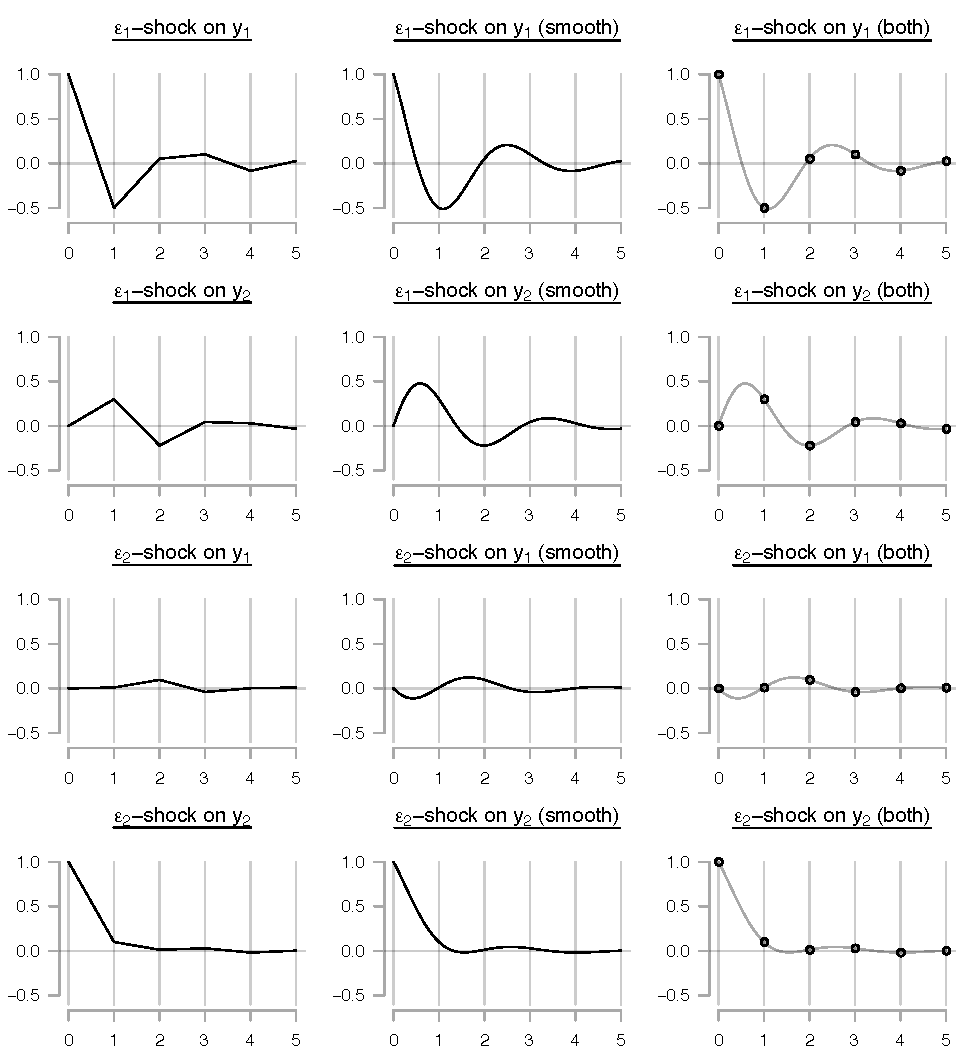
\includegraphics{graphs/numeric.pdf}
  \caption{Impulse Response Functions from Section~\ref{S3}
    example; $y_t$ is generated by Equation~\eqref{eq:10}. The left
    column plots standard \IRF s and the right column plots our new
    method.}
  \label{fig:3}
\end{figure}

We plot the \IRF s in Figure~\ref{fig:3}. The first column plots the
standard \IRF s and the second plots our proposed smooth
plots. Although the general impressions from both graphs are similar,
there are important differences. First, peaks and troughs are often
underestimated by the standard \IRF s and their timing is frequently
misidentified. This is especially apparent in the first peak in the
second row. Second, even the sign of the \IRF\ can be misidentified,
as we see with the immediate response of $y_{1t}$ to a shock in
$y_{2t}$. Finally, unless turning points in the smooth functions
happen to coincide with integer values, discretizing the \IRF s
introduces misleading asymmetries and kinks.

\begin{figure}[t]
  \centering
  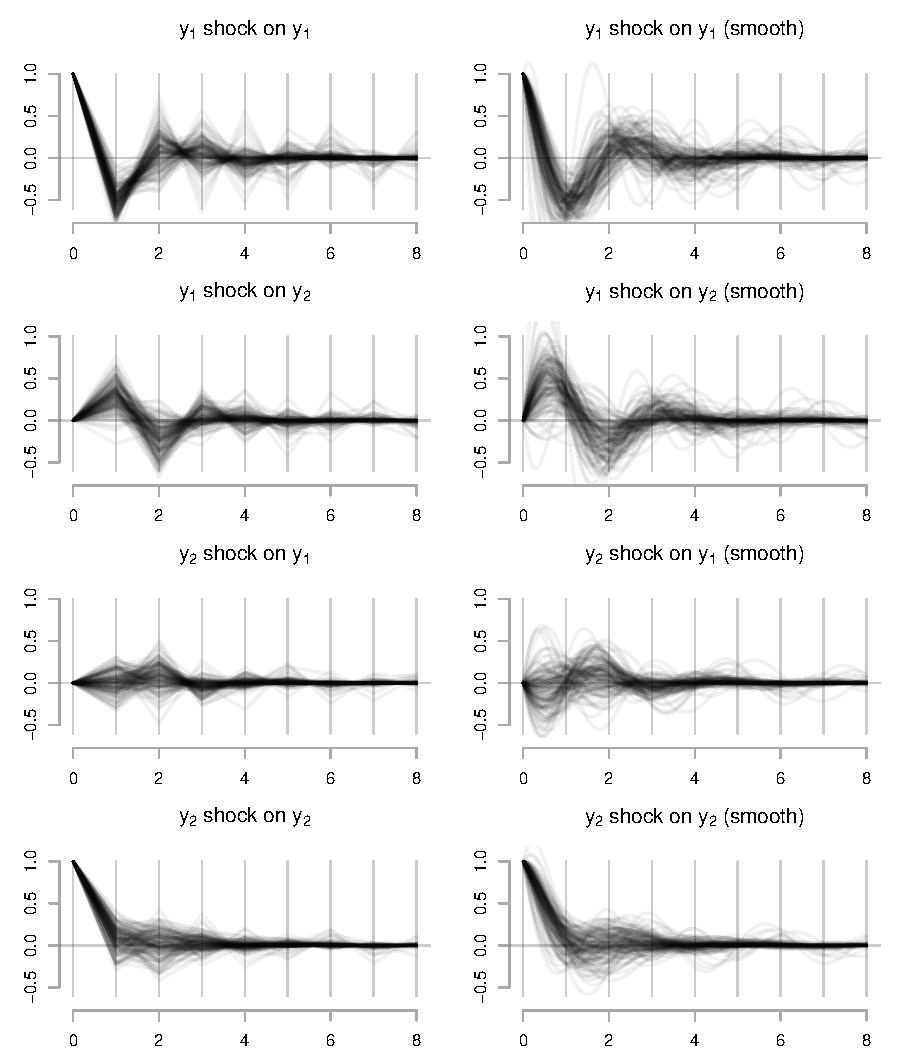
\includegraphics{graphs/numeric2.pdf}
  \caption{Impulse Response Functions from Section~\ref{S3}
    example; $y_t$ is generated by Equation~\eqref{eq:10}, with
    independent $N(0,0.15)$ random variable added to each
    coefficient. These graphs plot the \IRF s from 150 independent
    draws of the coefficient matrices. The left column plots standard
    \IRF s and the right column plots our new method.}
  \label{fig:4}
\end{figure}

These distortions are even more apparent when we graph multiple
perturbations of the \IRF s in the same panel, which is a common way
of representing uncertainty or set-identified responses. To
demonstrate this phenomenon, we generated 150 replications of the \IRF
s by adding independent N(0, 0.15) noise terms to each element of $A$,
and then plotting the implied \IRF s as before.

These graphs are shown in Figure~\ref{fig:4}. The same issues apparent in
Figure~\ref{fig:3} are present here as well. But there are other problems
as well. In the first curve, for example, the discrete \IRF\ shows
that there is substantial negative correlation between the period 2
and period 3 estimated response and the period 3 and 4 response. But
the smoothed graph makes it clear that this is driven by the timing
and size of the first peak. When that peak is near period 2, the curve
has time to fall noticeably before period 2, but when the peak is
closer to period 3, the curve is still rising for that interval. The
actual dynamics implied by the different curves are very
similar. Similar but less dramatic distortions appear in the other
panels as well. In the third row, for example, the discrete \IRF\
shows that about half of the parameter values have an initial increase
in response to a $y_{20}$ shock and half have an initial decrease, but
the smooth curves show that virtually all of them have an immediate
decrease, but that many start to increase very soon. The exact
location of the peak that falls between periods 1 and 2 determines
most of the initial dynamics, but this is impossible to see in the
discrete curve.

\section{Discussion}
\label{S4}

Vector Autoregressive models do not just have implications for the
period-to-period dynamics of a stochastic process, they also have
implications about the very short-run dynamics within periods. In this
paper, we propose that researchers graph those intra-period dynamics
when plotting \IRF s and we give a simple method to do so, based on
the \VAR's canonical \VAR(1) representation. Even when researchers do
not want to assign any economic importance to these ultra short-run
dynamics, plotting them in the \IRF s minimizes visual distortions
that can arise from discretizing the dynamics, especially when several
\IRF s are plotted over each other to represent uncertainty or set
identification.

\clearpage
\addcontentsline{toc}{section}{References}
\bibliography{latex_misc/references}

\clearpage
\appendix
\section{Appendix: Changes to this paper from previous versions}
\begin{description}
\item{Latest:}
  \begin{itemize}[noitemsep]
  \item Rerender pictures to fix display problems in some pdf vieweres.
  \end{itemize}

\item{v0.3, 2016-03-28:}
  \begin{itemize}[noitemsep]
  \item Makes small wording changes to the abstract.
  \item Changes the title of the paper.
  \item Adds empirical analysis of monetary policy (as in Uhlig, 2005).
  \item Adds Git commit information to the pdf.
  \item Adds this changelog to the pdf.
  \item Adds a table of contents to the pdf.
  \item Makes several small formatting changes.
  \item Makes several small changes to the internal file organization.
  \end{itemize}

\item{v0.2.2, 2015-02-22:} Tweaks the abstract.

\item{v0.2.1, 2015-02-21:} Adds author affiliation.

\item{v0.2.0, 2015-02-21:} Adds cumulative response function and VECM section; and
  revises the text of the paper.

\item{v0.1.0, 2015-02-11:} First draft of the paper.
\end{description}

%%% Local Variables:
%%% mode: latex
%%% TeX-master: "smoothirf.tex"
%%% TeX-command-extra-options: "-shell-escape"
%%% End:

\end{document}

%%% Local Variables:
%%% mode: latex
%%% TeX-master: t
%%% TeX-command-extra-options: "-shell-escape"
%%% End:
